The term Layer 2 refers to a series of blockchain solutions built on a different network running on top of layer 1, the main Ethereum network, through smart contracts. They are designed to increase the scalability of layer 1 while still being able to benefit, to some extent, from the security and the existing architecture of the Mainnet. The main idea for these protocols is to perform transactions off-chain to achieve a faster confirmation time, lower fees, and traffic reduction on the Mainnet. \cite{gudgeon_sok_2020, noauthor_layer_nodate}. 

For the reader's reference, a detailed list on the different solutions is available in appendices \ref{appendix:layer2:solutions} and \ref{appendix:layer2:examples}. The aim of these appendices is to systematise the panel of layer 2 protocols that emerged in the past decade. To this end, we provide a comparison of the main solutions in terms of structure, synchronisation with layer 1, scalability power and security.

One of the main drawbacks (\cite{0xjim_layer_2021}) of layer 2 solutions is that the system doesn't live on layer 1, it cannot interact with layer1 at a cheap cost. Lots of interesting projects (OpenSea, Uniswap, Aave ...) are not present on all second layers. Combining multiple Defi protocols is nearly impossible when using layer 2. For example, Aave is only available on Polygon, and Uniswap on the main network and Optimism. Thus, it is impossible to create an operation that uses Aave’s and Uniswap’s smart contracts. Liquidity also suffers from the presence of multiple layers. Indeed, the liquidity is split across layers and does not flow easily from one to another.

According to the scalability trilemma (cf. figure \ref{scalability-trilemma}), systems cannot achieve all of the following aspects: scalability, security and decentralisation. It means that if a solution performs well regarding scalability and security, it will have decentralisation shortfalls.
Lastly, as long as a decent amount of people keeps using the Ethereum main network, gas fees volatility will persist, regardless of second layers.


\begin{figure}[htbp]
    \centerline{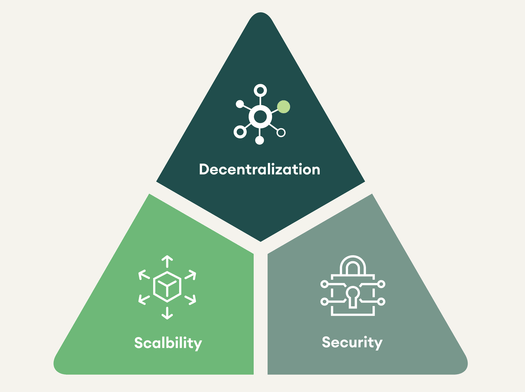
\includegraphics[width=60mm]{figures/scalability-trilemma.png}}
    \caption{Blockchain scalability trilemma \cite{BlockchainTrilemma}}
    \label{fig:scalability-trilemma}
\end{figure}


% no unified consensus
% security => do not use the same level of security as ethereum
% no do solve the gas fee problem  => still possible to hedge gas fees price on layer 1 

%%%%%%%%%%%%%%%%%%%%%%%%%%%%%%%%%%%%%%%%%%%%%%%%%%%%%%%%%%%
%%%%%%%%%%%%%%%%%%%%%%%%%%%%%%%%%%%%%%%%%%%%%%%%%%%%%%%%%%%
%%%%%%%%%%%%%%%%%%%%%%%%%%%%%%%%%%%%%%%%%%%%%%%%%%%%%%%%%%%


Ultimately, we conclude with a proof of need to show that {\projectName} brings novelties not captured by the panel of existing layer 2 solutions.

% why Refees is needed when all this pannel of layer 2 solutions is available in the market ?
